\section{III-THIẾT KẾ VÀ TRIỂN KHAI}
% Slide 1: Kiến trúc tổng quan
\subsection{Tổng quan kiến trúc}

\begin{frame}[fragile]{Kiến trúc Hệ thống FDAS}
    \begin{columns}[t]
        \begin{column}{0.5\textwidth}
            \begin{figure}
                \centering
                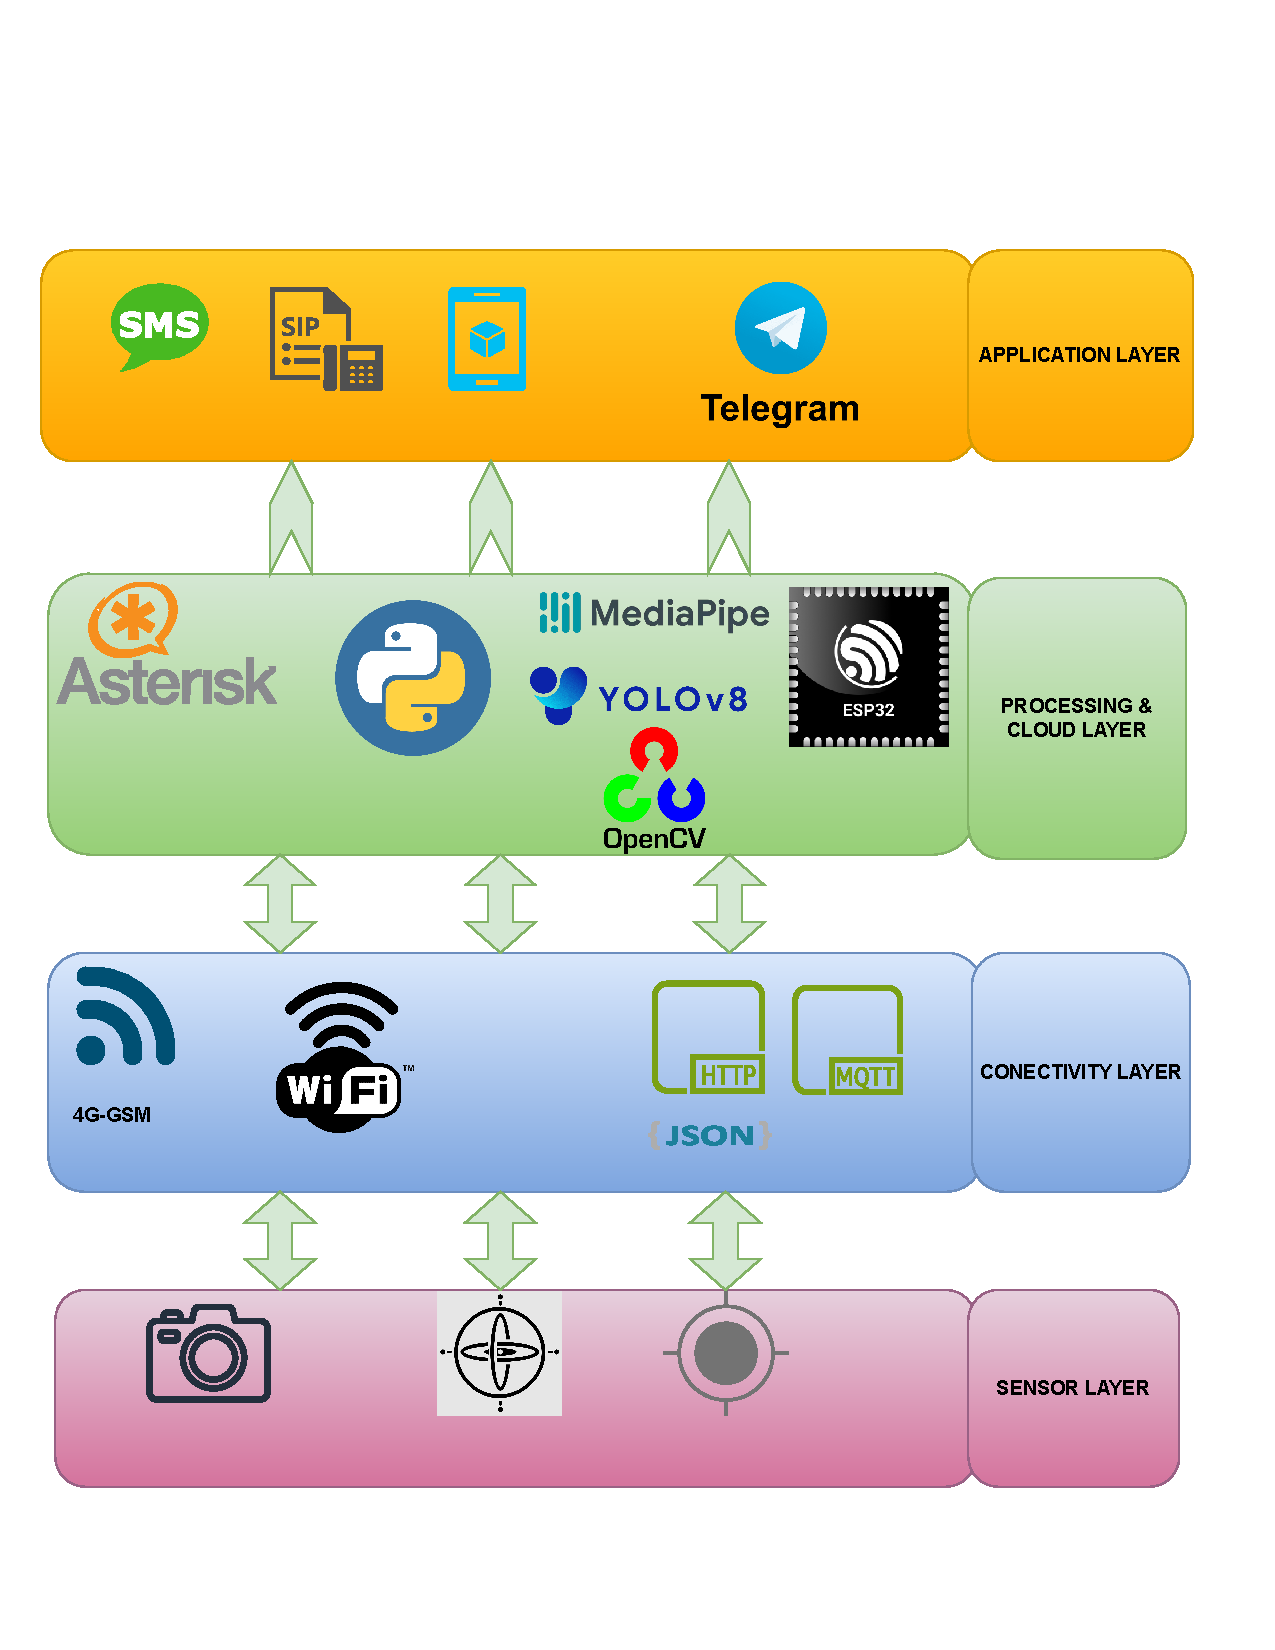
\includegraphics[width=0.85\textwidth,height=0.8\textheight,keepaspectratio]{images/system_architecture_diagram.pdf}
            \end{figure}
        \end{column}
        \begin{column}{0.5\textwidth}
            \begin{block}{Quy trình}
                \begin{itemize}
                    \item Minh họa kiến trúc hệ thống phát hiện té ngã và cảnh báo.
                \end{itemize}
            \end{block}
            \begin{block}{Mô tả}
                \begin{itemize}
                    \item \textbf{Lớp Thiết bị/Biên}: Thu thập dữ liệu.
                    \item \textbf{Lớp Kết nối}: Truyền tải dữ liệu.
                    \item \textbf{Lớp Xử lý/Đám mây}: Xử lý và ra quyết định.
                    \item \textbf{Lớp Ứng dụng/UI}: Giao diện người dùng.
                \end{itemize}
            \end{block}
        \end{column}
    \end{columns}
\end{frame}
% Slide 2: Lớp Thiết bị/Biên
\begin{frame}
\frametitle{Lớp Thiết bị/Biên}

\begin{columns}
\column{0.5\textwidth}
\begin{block}{ESP32 Module}
\begin{itemize}
\item Cảm biến gia tốc \& con quay
\item Phát hiện mẫu chuyển động té ngã
\end{itemize}
\end{block}

\begin{block}{Module GPS}
\begin{itemize}
\item Thu thập vị trí địa lý
\item Hỗ trợ giám sát ngoài trời
\end{itemize}
\end{block}

\column{0.5\textwidth}
\begin{block}{IP Camera}
\begin{itemize}
\item Luồng video liên tục
\item Giám sát trong nhà
\end{itemize}
\end{block}

\vspace{1cm}
\begin{alertblock}{Đặc điểm}
2 nguồn dữ liệu độc lập
\end{alertblock}

\end{columns}

\end{frame}

% Slide 3: Lớp Kết nối
\begin{frame}
\frametitle{Lớp Kết nối}

\begin{columns}
\column{0.5\textwidth}
\begin{block}{Kênh truyền}
\begin{itemize}
\item Wi-Fi/4G/LTE
\item Đảm bảo kết nối liên tục
\end{itemize}
\end{block}

\column{0.5\textwidth}
\begin{block}{MQTT Broker}
\begin{itemize}
\item Mô hình Publish/Subscribe
\item ESP32 → JSON data
\item Server nhận real-time
\end{itemize}
\end{block}
\end{columns}

\end{frame}

% Slide 4: Lớp Xử lý/Đám mây
\begin{frame}
\frametitle{Lớp Xử lý/Đám mây}

\begin{block}{Main Processing Server (Python)}
\begin{itemize}
\item \textbf{MQTT Client}: Subscribe dữ liệu từ ESP32
\item \textbf{AI \& Image Processing}: YOLO model xử lý video
\item \textbf{Business Logic}: Kết hợp 2 luồng dữ liệu → Quyết định cảnh báo
\end{itemize}
\end{block}

\begin{columns}
\column{0.5\textwidth}
\begin{block}{Asterisk Server}
\begin{itemize}
\item Tổng đài PBX
\item Cuộc gọi khẩn cấp (SIP)
\end{itemize}
\end{block}

\column{0.5\textwidth}
\begin{block}{Telegram Bot API}
\begin{itemize}
\item Tin nhắn/hình ảnh
\item Thông báo nhóm
\end{itemize}
\end{block}
\end{columns}

\end{frame}

% Slide 5: Lớp Ứng dụng/UI
\begin{frame}
\frametitle{Lớp Ứng dụng/Giao diện}

\begin{columns}
\column{0.33\textwidth}
\begin{block}{Mobile/Web App}
\begin{itemize}
\item Dashboard
\item Lịch sử sự kiện
\item Cấu hình
\end{itemize}
\end{block}

\column{0.33\textwidth}
\begin{block}{SIP Client}
\begin{itemize}
\item Linphone/Zoiper
\item Nhận cuộc gọi báo động
\end{itemize}
\end{block}

\column{0.33\textwidth}
\begin{block}{Telegram}
\begin{itemize}
\item Thông báo trực tiếp
\item Tương tác 2 chiều
\end{itemize}
\end{block}
\end{columns}

\vspace{0.5cm}
\begin{center}
\textbf{Cảnh báo đa kênh}: Gọi thoại + Nhắn tin
\end{center}

\end{frame}

